\section{Introduction}
\label{sec:introduction}
%
The GIPER instrument consortium answer to the ESA \ac{AO}\cite{JUICE_AO} for the L1 class \ac{JUICE} mission.
%
%
\subsection{JUICE Mission Overview}
ESA L1 mission selected May 2012 in Cosmic Vision programme. Expected launch date 2022. 7.5 year cruise to Jupiter. Orbit insertion 2030 around Jupiter including phase studies of Europa and Callisto. September 2032 orbit insertion around Ganymede. Nominal mission end 2033. Russian Ganymede lander.
%
%
 
\section{Scientific Objectives}
%scientific investigation. Overall instrument capability, global mission goal, anticipated scientific performance on instrument, compared to similar instruments, discussion of synergies between different observations, list of assuptions for achieving science objectives: SC performance, orbit, other payloads, ground segment.
%
The scientific outcome of this instrument proposal is in accordance with ESA \ac{SciRD}\cite{SciRD} and addresses many of the scientific investigations proposed in the ESA JUICE Assessment Study Report\cite{yellowbook}.
%
%

\subsection{Introduction \label{sub:Introduction-science}}

Ganymede is the largest moon in the Jovian System and one of the four
Galilean moon. It was discovered in 1610 by Galileo Galilei. With
a mean radius of 2634~km Ganymede is the largest moon in the Solar
System and even larger than the planet Mercury. It travels around
Jupiter in an orbit with a semi-major axis of $1070400$~km and an
eccentricity of 0.00013. It is therefore the third of the Galilean
moons. 

It is believed that Ganymede consists mainly of 3 layers which are
fully differentiated. The core consists of a hot iron alloy which
is responsible for generating the intrinsic magnetic field. The second
layer is made of heavier rocky material and the third layer consists
mainly of water ice. The icy surface is expected to be around 800~km
thick. On the boundary between the icy and the rocky layer large oceans
of liquid water may be present.


\subsubsection{The surface composition of Ganymede}

The main understanding of the surface composition and the underlying
processes of forming Ganymede originates from the Galileo mission
from 1989 to 2003. The objective of the Galileo mission was to investigate
the Jupiter system. Therefore most instruments were focusing on imaging,
measuring particles and fields and no subsurface measuring instrument
was available. An image of the Ganymede surface taken from the Galileo
orbiter is show in figure \ref{fig:Ganymed-true-color}. It consists
mainly of water ice and is basically separated into regions with a
low albedo, often referred to as dark terrain, which covers about
35~\% of the surface and regions of high albedo, named bright terrain
respectively, which covers 65~\%. The boundaries between dark and
bright terrain are sharp and distinct. The dark terrain is covered
with a much higher amount of impact craters. It is therefore believed
to be much older than the bright terrain%
\begin{comment}
dates missing
\end{comment}
. Stereo images suggests that the dark furrow terrain is generally
higher than the grooved bright terrain. This leads to the idea that
bright terrain has probably formed by tectonic processes of the (former)
dark terrain together with transport processes of snow or water to
the surface like cryo-volcanism (see also section \ref{sub:volcanism})
thereby smoothing the surface. Impact craters of meteoroids therefore
show up as bright white spots on the white terrain. 

\begin{figure}
\begin{centering}
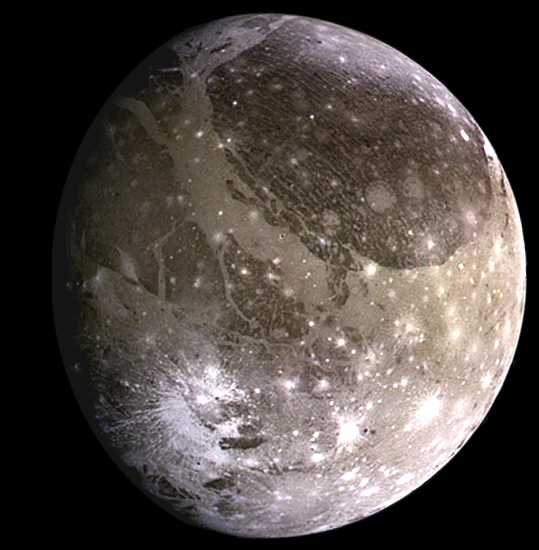
\includegraphics[width=0.70\textwidth]{Figures/Ganymede_true_color}
\par\end{centering}

\caption{\label{fig:Ganymed-true-color}}


\end{figure}



\subsubsection{Formation of the surface and sub-surface processes\label{sub:volcanism}}

The processes causing the formation of the bright terrain from the
ancient dark terrain are believed to be tectonics and cryo-volcanism
although they are still not fully understood and part of active discussions%
\begin{comment}
ref
\end{comment}
. Most models need a heat source strong enough to (partly) melt sub-surface
layers. The current orbital parameters of Ganymede would not be sufficient
to produce enough heat by tidal forces, orbital calculations suggest
that Ganymede had a period where the eccentricity of its orbit reached
as high as 0.03 %
\begin{comment}
ref
\end{comment}
{} which would cause enough tidal heating to melt parts of the icy interior. 

Another unknown problem is the transport of the then (partly) molten
ice or slush to the surface in order to fill graben. One proposition
is that icy ,,volcanoes`` ejected low-viscous liquid water which
then flooded the graben before freezing. So far no strong evidences
for this volcanism like downstream patterns on the horsts or ejection
centers. This may be because the resolution of the images obtained
by the Galileo and Voyager missions do not have a high enough resolution,
the areas for which high resolution pictures are available do not
have pronounced enough evidences or there are just not existent%
\begin{comment}
ref
\end{comment}
. Another problem is that water or slush have a higher density than
ice thus if tidal heating would melt ice the water or slush would
sink deeper instead of rising to the top.

An approach to solve this issue which would also explain why there
is no ice on top on the horsts and the lack of flooding tracks is
that tectonics resurfaced the dark terrain to contain horsts and grabens.
These apply different pressure to the underlying terrain. These pressure
gradients could actually lead to the circumstance that material with
a negative buoyancy like water or slush could move upwards but only
below the grabens. When the graben are filled with ice, the process
automatically stops because the necessary pressure imbalance from
the terrain disappears hence no ice could reach the high horsts%
\begin{comment}
ref
\end{comment}
. 

In figure \ref{fig:gradients} an example calculation for the gradients
due to terrain imbalance is presented. The terrain was modeled as
a sine wave with 30~km wavelength and an amplitude of 1~km (2~km
peak-to-peak) as shown in the top graphic of figure \ref{fig:gradients}.
\begin{figure}
\begin{centering}
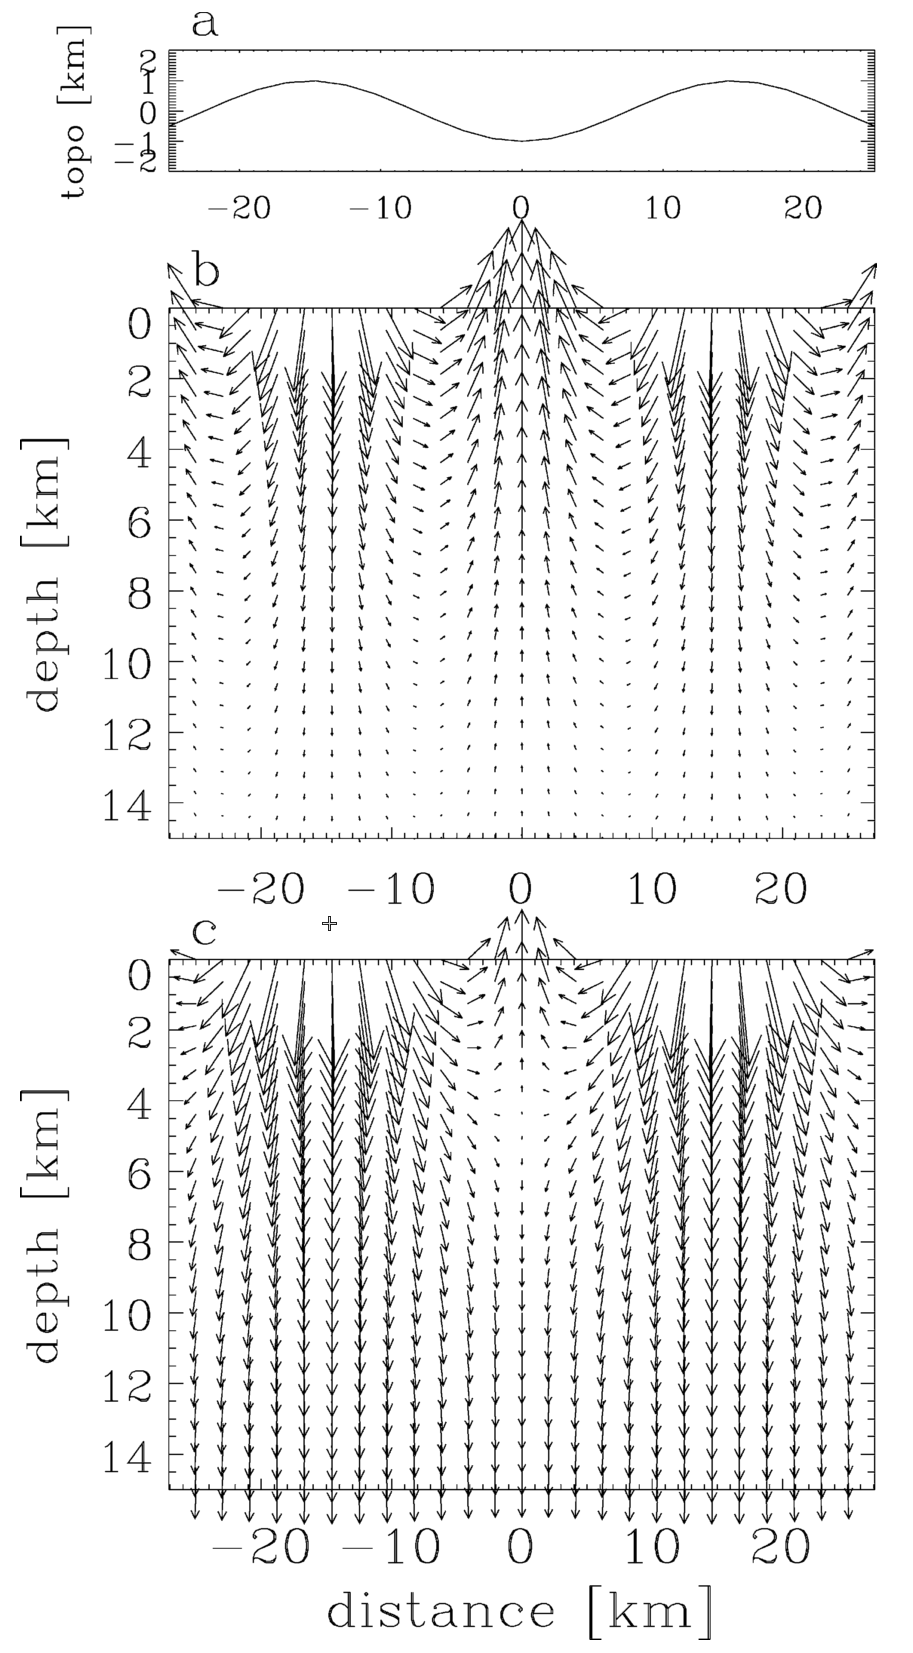
\includegraphics[width=0.70\textwidth]{Figures/gradients}
\par\end{centering}

\caption{\label{fig:gradients}}


\end{figure}
 The vector plot in the middle shows the resulting pressure gradients.
As can be seen underneath the graben they are directed upwards but
decrease exponentially with depth. The lower vector plot shows the
resulting gradients when considering water with a negative buoyancy.
As can be seen water could only move up to the surface when it is
created in a depth below 5~km. Further calculations performed by
Showman, Mosqueira et al. estimate that depth from where water or
slush can rise to the surface ranges from 5~km to 10~km. A possible
problem with this model may be that is would need at lease 1 million
years to transport enough water to the surface in order to fill grabens,
but the graben could relax gravitationally earlier and thus stop the
upward flow. 

In order to find the dominant processes for the resurfacing of Ganymede's
dark terrain it would be essential to acquire measurements from the
subsurface interior additionally to (new) surface pictures. Ganymede
can be seen as a prototype for an icy body. Therefore investigating
the tectonic processes of Ganymede and its surface evolution will
not only provide more information about the formation of Ganymede
but also of its siblings Europa and Callisto as well as icy bodies
in general %
\begin{comment}
ref 
\end{comment}
.


\subsection{Scientific Goals\label{sub:Scientific-Goals}}

Based on the short scientific introduction of Ganymede from section
\ref{sub:Introduction-science} the following scientific goals can
be identified:
\begin{itemize}
\item Map the interior below the surface of Ganymede to get more insight
about different layers and their composition. 
\item Find evidences for the tectonic processes which created the horsts
and grabens of the grooved terrain
\item Find evidences for or against different cryo-volcanism scenarios
\item Get a more detailed map of the surface terrain compared to stereoscopic
imaging
\item Possibility to find habitable zones 
\item yada yada yada
\end{itemize}

\subsection{Scientific Performance Requirements}

In order to achieve the goals described in section \ref{sub:Scientific-Goals}
the instrument should be able to penetrate the surface to at least
5~km. Attenuation of radar waves in the lower MHz spectrum in ice
is quite small which is beneficial for a high penetration depth, but
although it is quite certain that the upper surface mainly consists
of water ice there might be significant amounts of rocky material
at some parts due to the many meteoroid impacts after the accretion
phase of Ganymede. Therefore an appropriate margin for the penetration
depths should be considered. 

The vertical resolution should be in the range of 10~m -- 35~m to
give the chance to resolve the position and offset of the identified
layers with high accuracy. A typical width for the groves of the terrain
is 10~km, thus the horizontal resolution should not exceed this value
in order to correlate different vertical layers to the surface terrain. 

As the goal is to create a map of the whole surface of Ganymede it
is expected that even after preprocessing and compression a large
amount of data will be collected. An appropriate downlink capacity
should be reserved for the mission.


\section{Technical Description and Design}
%
The proposed instrument has been designed in accordance to ESA \ac{EID-A} for the \ac{JUICE} mission\cite{EIDA}.
%
\subsection{Design Overview}
\subsection{Instrument Design Elements}
\subsection{Technical Resources}
\subsection{Instrument Spacecraft Requirements}
%thermal, power, mechanical mounting, EMC, especially radiation sensitive parts, radiation shielding and mitigation strategy, flight heritage of hardware, ressource budgets, 
This mission assumes that an altimeter instrument is included in the JUICE mission scientific instrument package. Altimeter is needed to estimate the surface clutter and surface slope.
%
\section{Summary of Instrument Interfaces}
%data, mechanical, power, EMC, thermal,
%
\section{On-ground and In-flight Test and Calibration}
%test equipment requirements (i.e. thermal vacuum chamber, EMC labs etc.), EGSE, radar signal simulator(test of ground processing chain),
%
Functional, EMC, Thermal-Vacuum, Vibration.
%
%
For \ac{EGSE} a \ac{GIPER} raw signal simulator will be developed by the instrument consortia. The raw signal simulator will be similar to the one developed for the \ac{SHARAD} instrument\cite{Giovanni} and allow testing of the signal processing chain and to develop a Ganymede transfer function considering the orbit altitude and surface clutter and sub-surface dielectric interfaces. 
%
%
\begin{wrapfigure}{r}{0.3\textwidth}
\centering
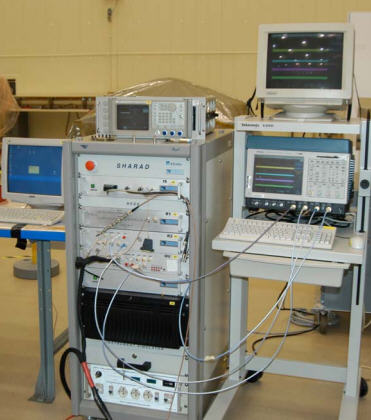
\includegraphics[width=0.27\textwidth]{Figures/MEGS}
\caption[caption]{Mars Echo Generation System used on the SHARAD instrument\cite{MEGS}}
\label{fig:MEGS}
\end{wrapfigure}
%
%
In-flight internal calibration (transmitted signal looped to receiver and data sent to ground)
In-flight external calibration (unprocessed data of reflected signals from a flat surface region of Ganymede is sent to ground)
%
%
\section{System Level Assembly, Integration and Verification}
%
%
\subsection{Requirements}
\subsection{Deliverable Models}
%
Two models of the proposed instrument will be developed:
\begin{itemize}
\item Engineering Model - To test and verify the instruments functional and technical requirements as well as the instrument performance.\\
\item Protoflight Model - will be build using full flight standard components and tested at qualification levels.
\end{itemize}
%
\subsection{System Level Testing}
%
\section{Flight Operations Concept}
%operational modes, calibrations, 
%
The instrument modes are inherited from the SHARAD instrument\cite{SHARAD_ppt}.
%
\subsection{Nominal Operations}
%
Operation modes: Low data rate, high data rate, calibration, receive only
%
\subsection{Other Modes}
%
Silent Modes: Off, Heating
Support modes: Check/init, standby, warm-up, idle
%
%
%
\section{Science Ground Segment Concept}
%operations requests, on-board software maintenance (test facilities to generate and test update)
%Further described in the Science Implementation Plan (SIP) - answer to SIRD
%
\section{Data Reduction, Scientific Analysis and Archival Plans}
%
\section{Organization}
%\subsection{Schedule}
\subsection{Management Structure}
(Please note, some of the contents in this section are fictive and should not be taken literally.)\\\\
%
\noindent
Dr. Jan Sommer is the instrument \ac{PI}. He has an extensive background studying planet geology, especially on Mars. This study will enhance our knowledge of planet inner structures, geology and provide better understanding of planet formations and evolution.\\\\
%
\noindent
Morten Olsen is the project manager. With experience as project manager for previous successful space instruments, he will manage the project schedules and budgets.\\\\
%
\noindent
Omair Sarwar is the technical manager. With extended engineering experience in radar systems, he will ensure that the instrument meets the performance requirements, proper instrument verification and qualification in accordance with ESA space standards.\\\\
%
\subsection{Budget}
ACME Space Agency is the \ac{LFA} for this instrument proposal. A \ac{LEO} has been issued ensuring funding for the project during the instrument development phase, in-flight operations and post operations activities.